\documentclass[sigconf,nonacm]{acmart}

% enable links
\usepackage{hyperref}
% larger page margins

\usepackage{subcaption}
\usepackage[font=small,labelfont=bf,textfont=md]{caption}
\usepackage{graphicx}
\usepackage{multirow}

\begin{document}

\title{Exploring and Analyzing Compression Algorithms in Preprocessing Pipelines}

\author{Adrian David Castro Tenemaya}
\email{adrian.castro@tum.de}
\affiliation{%
  \institution{Technische Universit{\"a}t M{\"u}nchen}
}

\begin{abstract}
  End-to-end training pipelines nowadays take a lot of time to train due to the rise in model size and the amount of data needed to feed them.
  Most recent literature focuses on ways to optimize the model training phase, ignoring preprocessing and data handling times in both local and distributed environments.
  However, preprocessing may take up to 45\% of the total time in end-to-end training pipelines.
  Compression algorithms have proven to be useful in several areas to reduce I/O network bandwidth and storage consumption.
  In turn, the use of compression leads to additional processing power overhead during compression and decompression stages.
  It is crucial then to analyze and select appropriate compression strategies depending on the environment, with the goal to find a good balance between compression ratio and speed.
  
  In this work, we show the integration of the Zstandard compression library into the popular machine learning library TensorFlow.
  We further explore and analyze the effects of data compression on storage and network usage with respect to deep-learning preprocessing pipelines.
  We also show the impact of different compression options for GZIP and ZLIB compared to default parameters.
  Lastly, we include observations regarding the impact of different compression algorithms on several datasets and data types (e.g. JPEG vs. PNG).
\end{abstract}

\maketitle

\section{Introduction}
Deep learning is data and computationally intensive, with end-to-end workflows possibly taking weeks or months to complete.
Besides, neural networks are trained on expensive dedicated hardware such as GPUs and TPUs to reduce training times.
Training can either happen on-premise or on the cloud.
The cost of training is generally calculated depending on the time spent using the devices.
Because of this, practitioners and researchers have to find ways to maximize their usage in terms of computational power and minimize the amount of time spent training them.

Over the past few years, research in this area has been focused on the optimization of the model training phase, with techniques such as data and model parallelism being the most used.
This has allowed deep learning workflows to scale horizontally to models with billions of parameters \cite{smith2022deepspeed}.
With the increase in computational power, data ingestion and preprocessing pipelines need to keep up with the high amount of throughput needed to keep the training hardware as busy as possible.
Recent research has shown that these types of pipelines can take up to approximately 45\% of the total end-to-end training workflow time \cite{xin2021productionml}.
However, the development of techniques and frameworks trying to optimize data preprocessing and ingestion is limited, receiving little to no attention in research.

Recent work \cite{isenko2022bottleneck} has shown potential space for improvement in this area.
For example, applying certain transformations during the preprocessing phase may decrease data size.
If the dataset then fits into memory, network I/O bottlenecks can be severely decreased due to most operations now happening locally.
The use of lossless compression algorithms in preprocessing pipelines has been found to increase throughput under certain conditions.

We reproduced the results shown in \cite{isenko2022bottleneck} and found that the compression algorithms used may increase throughput.
However, this comes at a high cost in terms of processing time.
ZLIB has several strategies that perform differently according to how data is represented on disk.
If not selected, ZLIB defaults to \texttt{Z\_DEFAULT\_STRATEGY} as its compression strategy.
In this paper, we further investigate the effects of ZLIB and its different strategies on the same datasets and pipelines as \cite{isenko2022bottleneck} using the PRESTO library.

The \texttt{DEFLATE} compression algorithm, used by both ZLIB and GZIP, is quite old and does not reflect current advances in technologies and system architectures.
Intuitively, more recent compression algorithms may behave differently and perform better on the same datasets.
Zstandard \footnote{https://facebook.github.io/zstd/} is a lossless compression algorithm developed by Facebook in 2015 and has gained a lot of traction amongst practitioners for its speed and high customizability.
We decided to run the same experiments using Zstandard and compared the results against other compression algorithms and strategies.
However, TensorFlow's \texttt{TFRecord} only supports GZIP and ZLIB.
As part of our work, we created a custom TensorFlow implementation to include the lossless compression algorithm Zstandard.
Our analysis reveals that Zstandard decreases compression and decompression overhead times by up to $81\%$ compared to GZIP and ZLIB in all scenarios.

In this paper, we argue that the selection of a compression algorithm is crucial to minimize compression and decompression overhead and potentially maximize throughput.
We further analyze the challenges arising from the implementation of compression in deep learning preprocessing pipelines.
In particular, we present what we have learned about the current state-of-the-art regarding the use of compression algorithms in deep learning and their impact on training.
Finally, we showcase possible suggestions regarding the use of compression in preprocessing pipelines.

\section{Setup and background}
We start by describing the setup that was used to perform the tests.
Our experiments were run using a virtual machine with 40GB DDR4 DRAM, 16 VCPUs on an Intel Xeon E5-2630 v3 16x@2.4 GHz with an Ubuntu 18.04 image on our OpenStack cluster.
We use a Ceph cluster as our main storage, backed by HDDs, with a 10 Gb/s uplink and downlink.
Ceph is used for storing the intermediate dataset representations and the unprocessed datasets.
We repeat each experiment five times, and we drop the page cache after every run to remove memory caching effects.
All experiments are run with 8 threads and are executed with Python 3.7 and TensorFlow 2.7.
We included Zstandard 1.5.0 in all experiments that extended \texttt{TFRecord}.

\subsection{Datasets}
For our experiments, we decided to stick to 4 out of 6 of the datasets analyzed by \citet{isenko2022bottleneck}.
A detailed list of properties of these datasets is represented in \autoref{table:datasets}.

\begin{table*}
  \centering
  \begin{tabular}{ |c|c|c|c|c|c|c|c| }
    \hline
    Dataset name                                & Samples & Size in GB & \multicolumn{4}{c|}{Steps}                                                                     \\
    \hline
    Cube++ PNG  \cite{ershov2020cube++}         & 4890    & 85.17      & 2-read-image               & 3-decode-image           & 4-resize-image & 5-center-pixel-values \\
    Cube++ JPG  \cite{ershov2020cube++}         & 4890    & 2.54       & 2-read-image               & 3-decode-image           & 4-resize-image & 5-center-pixel-values \\
    Librispeech \cite{panayotov2015librispeech} & 28K     & 6.61       & 2-read-and-decode-flac     & 3-convert-to-spectrogram &                &                       \\
    Commonvoice \cite{ardila2019commonvoice}    & 12K     & 0.25       & 2-read-and-decode-mp3      & 3-convert-to-spectrogram &                &                       \\
    \hline
  \end{tabular}
  \caption{List of datasets used for this paper, with number of samples and preprocessing steps.}
  \label{table:datasets}
\end{table*}

\subsection{A Brief History of Compression Algorithms}
Data compression algorithms have been used almost since the very beginning of telecommunications. A very early example is Morse code.
Common English letters ``e'' and ``t'' are abbreviated with shorter code words, hence, achieving compression when communicating those letters over long messages.
During the late 1970s, with the early development of inter-machine communication over cable came the need to reduce the storage footprint of data and communication overhead, officially kick-starting research into compression algorithms.

We have two macro-types of compression algorithms: \textit{lossless} and \textit{lossy} compression algorithms.
The former can be applied to input data to reduce its size, and the result can later go through a process called \textit{decompression}, which restores the original input without any loss of information.
The latter is still applied to input data to reduce its size, but in such a way that some original information is lost, and recovering the original input is not possible.

The first compression algorithms were lossless, using the well-known Huffman Coding, invented by David Huffman in 1949.
Today, Huffman Coding is still being used in almost every lossless compression algorithm.
Most modern lossless compression algorithms, such as LZ77 \footnote{Lempel-Ziv, 1977} and LZW \footnote{Lempel-Ziv-Welch, 1984}, started to show up later in the century.

Lossy compression algorithms are a more vague categorization.
Image cropping, rotation, down-scaling, and other operations can be seen as examples of lossy compression, as the application of these functions has a result that may not retain all the input's original information.
In medical applications, for example, x-rays are generally represented as gray-scale pictures.
For this reason, every pixel does not need to be represented by three channels, but just one, with a potential 3x saving in terms of storage space.
Lossy compression algorithms have everyday life applications: audio formats (MP3), image formats (JPEG), and more.

In general, compression is used across a wide array of topics.
When surfing the web, HTML pages are probably compressed using either GZIP or brotli, and pictures are either losslessly compressed (PNG) or lossy compressed (JPG).

\subsection{Preprocessing Pipelines}
The preprocessing pipeline is a crucial component of end-to-end deep learning workflows, and defines how data should be acquired and consumed by the model before and during training.
They can be split into steps or operations, each either running once, called ``offline'' steps, or iteratively throughout training, called ``online'' steps.
The order and type of operations differ according to the type of DNN that is being trained and have a huge impact on a model's training performance and accuracy.
Offline steps are operations that are static and deterministic, such as image decoding and resizing.
Online steps instead are typically non-deterministic and augmentation operations, such as random image cropping or random brightness image augmentation.

Selecting the order of the steps in preprocessing pipelines is a complex task.
For this work, we stick to the step selection chosen by \cite{isenko2022bottleneck}.

\subsection{Distributed Storage}
To train deep neural networks, large amounts of data are needed.
Preprocessing pipelines need to provide the highest amount of throughput to accelerators to keep them as busy as possible.
This translates into the need to serve terabytes or even petabytes of data across the entire training workflow.
Network speeds are greater than most storage devices, even SSDs, by at least one order of magnitude.
At the time of writing, average network cards installed in servers can provide speeds of up to 100Gb/s, while high-end SSDs can reach speeds of up to 4-5Gb/s.
HDDs are even slower, with transfer rates topping 1.2Gb/s, but are also the cheapest viable option for large-scale storage.

Deep learning training generally involves repeatedly read and write operations on shuffled data.
However, if data is stored on hard disks, read operations need to perform random access to disks, a notably slow task.
Even if solid-state drives were used, speeds would not remotely come close to what a network connection can provide.

For a long time, parallelism techniques have made it possible to exploit high network speeds instead of just relying on sequential file storage access.
To achieve high performance in file intensive tasks, distributed storage solutions such as HDFS \cite{hdfs2010}, Ceph \cite{ceph2006}, TensorFlow \texttt{TFRecord} \footnote{https://www.tensorflow.org/tutorials/load\_data/tfrecord} and Amazon S3 \footnote{https://aws.amazon.com/s3/} exist.
Each one of these solutions has its own set of benefits and disadvantages, but employs similar approaches to how to store and serve data to achieve high-performance I/O over the network.
Files can be stored on different servers and then later be accessed by a client through the network, achieving higher speeds than sequential access.

In this paper, we employ a Ceph cluster as our main storage solution, with a 10Gb/s uplink and downlink.

\subsection{Related Work}
Efficiently managing computational resources, network I/O and storage consumption is especially important for Internet-of-Things (IoT), mobile, and edge devices.
Most of the time, it is not possible to control the hardware characteristics of the target devices, or to even know them.
In some cases, consumption and computational power may be bound to several orders of magnitude with respect to regular or dedicated devices.
This leads to the need to reduce the amount of computational power being used by algorithms, as well as storage consumption.

\textit{Compression techniques to reduce model size}.
Training and performing inference for deep learning models have typically much higher requirements in terms of computational power than regular IoT software.
As models get bigger, more computational power is needed to execute operations, more RAM to fit weights and runtime variables, and more storage to house data and the model itself.
Consequently, it is simply not possible to store and run state-of-the-art deep learning models, which may contain hundreds of millions, if not billions of parameters.
Compression techniques such as pruning and quantization have been applied to model weights to reduce their storage consumption and memory footprint \cite{song2015deep, davis2020pruning, torsten2021sparsity}.

While in this paper our main focus is on preprocessing pipelines, these issues are currently being tackled using not too dissimilar approaches.

\textit{Analysis of image compression formats impact on DNN accuracy}. It is fundamental to understand how compression algorithms affect a model's accuracy.
Images that may look similar to human vision can be fundamentally different at a data level.
In \cite{dodge2016understanding}, they analyze the effects of different artifacts in JPEG and JPEG-2000 on different computer vision pipelines.
According to their findings, models are more sensitive to Gaussian blur and noise with respect to compression level and contrast.
\citet{liu2018deepn-jpeg} present DeepN-JPEG, a JPEG-based image compression format tailored to DNN performance, while maintaining the same accuracy levels.

\textit{Data formats for fast I/O}. Different data representations on disk can affect access speed at runtime.
As shown by \citet{aizman2020highperformance}, practitioners do not necessarily need to come up with their own data format to achieve great speeds.
In their work, the old data format TAR is used by enforcing simple conventions on filenames and directory structure and iterated through their PyTorch client WebDataset.
The use of TAR makes their approach intriguing to researchers and practitioners, as it is widely supported across almost every system, and it is simple to integrate into already existing pipelines.

Very recently, the FFCV \cite{leclerc2022ffcv} PyTorch data loader entered the data loaders scene.
As shown by their experiments, it is able to speed up data loading times significantly, resulting in much lower prices for dedicated accelerators.
It can directly convert indexed PyTorch dataset formats as well as WebDataset.


\section{Extending TFRecordWriter}
In deep learning, we generally load files in batches, which are then consumed by dedicated hardware during model training.
File representation on disk plays a major role in how efficiently batches are loaded into memory, especially if data is stored on disk.
In this case, randomly accessing binary data can be extremely slow.
Google's TensorFlow provides the \texttt{TFRecord} file format to deal with these challenges, along with \texttt{tf.data} API to access it.
\texttt{TFRecord} can store several data points in a single or multiple binary files called ``shards''.
This limits random access to disk to a minimum, speeding up file reading from disk.
Benefits of sharding have already been studied previously in \cite{aizman2020highperformance}.

However, it is worth noting that storing files using \texttt{TFRecord} comes with the disadvantage that some preprocessing is needed.
Specifically, shuffling needs to take place prior to writing to disk, as \texttt{TFRecord} does not support random access.
These files can then be loaded in parallel, further speeding up read operations.

TensorFlow's release is 2.7, which is the version we started to work with at the beginning of the experiments, has \texttt{TFRecord} supporting GZIP and ZLIB as compression techniques.
\citet{isenko2022bottleneck} showed that these implementations are able to achieve higher data throughput under certain circumstances \cite{isenko2022bottleneck}.
They compare space-saving and throughput when applying compression to preprocessing steps.
When comparing JPG vs. PNG in the Cube++ dataset \cite{ershov2020cube++,ershov2020problems}, they found that the PNG pipeline results in much higher space-saving and throughput when compared to JPG.

These findings, they argue, may be explained by the fact that PNG is a losslessly-compressed file format, while JPG is lossy-compressed.
Converting from other image file formats to JPG introduces artifacts \cite{liu2018deepn-jpeg}.
These artifacts may negatively affect further compression when using ZLIB and GZIP \cite{isenko2022bottleneck}.
However, further tests are needed, and other compression algorithms need to be studied to confirm this behavior.

In our paper, we started by wanting to extend these findings by adding another lossless compression algorithm to compare GZIP and ZLIB on the same experiments as \cite{isenko2022bottleneck}.
To do this, we had to take a more in-depth look at how \texttt{TFRecord} writes to disk and how ZLIB and GZIP are integrated into it to decide which compression algorithm to experiment with.

\begin{figure}
  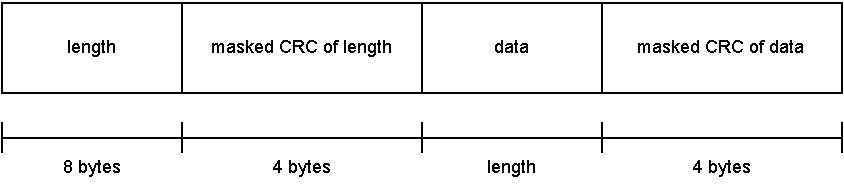
\includegraphics[width=\linewidth]{../images/TFRecord.pdf}
  \caption{The structure of a TFRecord.}
  \Description{}
  \label{fig:tfrecord}
\end{figure}

\texttt{TFRecord} binary files are a series of consecutive items, and every item inside contains a header, the actual data, and a footer (see ~\autoref{fig:tfrecord}).
When initializing a new \texttt{TFRecord}, an instance of the class \texttt{tensorflow::io::WritableFile} is created depending on the selected compression type, or its absence.
In the latter case, the writer class will just write contents to the file.
Instead, when a compression algorithm has been selected, every new item added to \texttt{TFRecord} gets compressed.

Typically, compression algorithms provide APIs to support two different cases: regular compression and streaming compression.
Regular compression, put simply, requires immediate knowledge and access to the whole input data and its original size.
This speeds up and improves compression ratio, and is generally the most common use case.
In some scenarios, however, access to all the information about a dataset is not immediately available.
This is the case when dealing with data streaming, as data flows at very high and irregular rates.
Streaming compression APIs are built exactly to deal with this problem.
Instead of compressing everything at once, an internal state is generally kept across compression runs.
This way, every time a new item needs to be compressed, previous information is not lost, and the compression rate improves.
Because \texttt{TFRecord} does not make assumptions about how big the original dataset is and allows users to programmatically add items to existing records, streaming APIs are used when performing compression.

Following these observations, we chose to add support for Zstandard (ZSTD) to \texttt{TFRecord}, using its Streaming API.
The library is written in C, and is being actively maintained.

\section{Experiments}
Over the years, compression algorithms have been invented and altered depending on the task at hand.
We devised our experiments to shed light on how different compression algorithms may affect preprocessing pipelines' performance.
We use the same datasets as \cite{isenko2022bottleneck}, described in \autoref{table:datasets}, with the exception for Openwebtext and ImageNet.
In the original paper, the number of runs per experiment is five.
However, for this work, the number of runs has been reduced to three times due to a change in specifications of the virtual machine that runs the experiments.

The compression algorithms we analyzed are ZLIB and ZSTD, with the following configurations:

\begin{itemize}
  \item \textbf{ZLIB compression strategies}. ZLIB uses \texttt{Z\_DEFAULT\_STRATEGY} as the default compression strategy, and it is reportedly good for general applications.
        However, there exist more strategies that presumably have better performance. %
        We experimented with different ZLIB compression strategies, namely: \\
        \texttt{Z\_FIXED}: prevents the use of dynamic Huffman codes. Instead, a fixed table is used \footnote{https://www.rfc-editor.org/rfc/rfc1951}; \\
        \texttt{Z\_FILTERED}: can be used for data produced by a filter, forcing more Huffman encoding and less string matching; \\
        \texttt{Z\_HUFFMAN\_ONLY}: forces Huffman encoding only, without string matching; \\
        \texttt{Z\_RLE}: specifically designed to give better compression for PNG data, but be almost as fast as \texttt{Z\_HUFFMAN\_ONLY} \footnote{http://optipng.sourceforge.net/pngtech/z\_rle.html}.
        It uses the Run-Length Encoding \cite{robinson1967results} as its main compression strategy, backed by a dynamic Huffman table.
  \item \textbf{ZSTD}. We implemented the ZSTD streaming API, using the default compression strategy for \texttt{ZSTD\_c\_strategy = 0}.
        Multithreading is not currently supported by our implementation but can be added in the future for possible speedups in a multithreading environment.
\end{itemize}

The compression level remained the default for both ZLIB and ZSTD, respectively at 6 and \texttt{ZSTD\_CLEVEL\_DEFAULT}.
\subsection{ZLIB}
ZLIB is a very common and general-purpose compression algorithm.
In its default strategy \texttt{Z\_DEFAULT\_STRATEGY}, it uses a balanced combination of Huffman Encoding and string matching to perform compression.
This is generally good for most applications, but in specific scenarios, it may overperform or underperform significantly.
We make the following observations based on \autoref{fig:zlib-experiments}:

\textbf{(1) Some strategies have similar performance}.
The compression strategies \texttt{Z\_RLE} and \texttt{Z\_HUFFMAN\_ONLY}, when compared, perform very closely to each other in terms of both speed and throughput.
The same effect can be seen for \texttt{Z\_DEFAULT\_STRATEGY}, \texttt{Z\_FILTERED} and \texttt{Z\_FIXED}.
This effect is not coincidental.

\texttt{Z\_RLE} comes with the advantages of \texttt{Z\_HUFFMAN\_ONLY}, as it only has to store the Huffman buffer and calculate the Huffman trees \cite{zlib2000zrle}.
\texttt{Z\_DEFAULT\_STRATEGY}, \texttt{Z\_FILTERED} and \texttt{Z\_FIXED} all use string matching, differing only in how they make use of Huffman encoding.
Note that both \texttt{Z\_RLE} and \texttt{Z\_HUFFMAN\_ONLY} have up to 1.4x higher throughput in the Cube++ PNG pipeline compared to no compression but lower throughput than other strategies.
In both the Cube++ JPG and Cube++ PNG pipelines, we can observe that \texttt{Z\_RLE} and \texttt{Z\_HUFFMAN\_ONLY} also execute much faster than \texttt{Z\_DEFAULT\_STRATEGY}, \texttt{Z\_FILTERED} and \texttt{Z\_FIXED}.

Interestingly, when looking at Librispeech and Commonvoice, all experimented algorithms show similar performance.
Furthermore, \texttt{Z\_RLE} and \texttt{Z\_HUFFMAN\_ONLY} are even able to outperform the absence of no compression, taking up to 80\% as much time.
These observations can help us understand how different approaches to data compression can affect how fast data is consumed.
In this particular case, the absence of string matching in both \texttt{Z\_RLE} and \texttt{Z\_HUFFMAN\_ONLY} can explain both the significant speed reduction and the lower throughput.

\textbf{(2) Storage savings are still not a predictor of throughput}.
Across every test we analyzed, we could not pinpoint a trend that may correlate storage savings and throughput.
We suspect that compression and decompression speed may play a major role in determining throughput.
However, we don't have specific data about these metrics, so more testing is needed.

\begin{figure}[b]
  % JPG
  \begin{subfigure}{0.49 \columnwidth}
    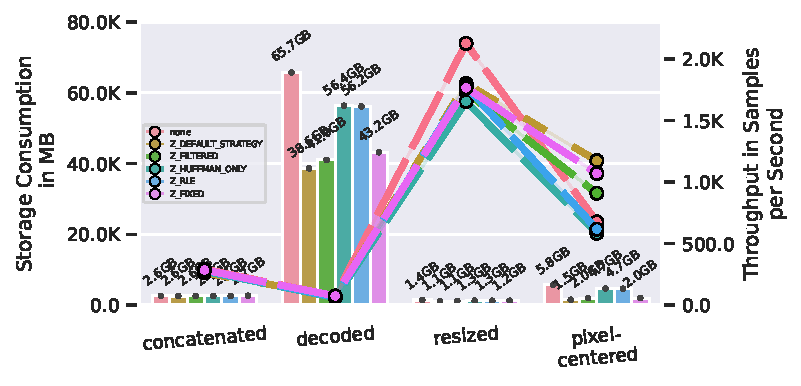
\includegraphics[width=\linewidth]{../images/cubeplusplus-jpg-strategy-pipeline/compressed-storage-vs-throughput.pdf}
    \caption{Cube++ - JPG}
    \Description{}
    \label{fig:zlib-cpp-jpg-compressed-storage-vs-throughput}
  \end{subfigure}
  \hfill %%
  \begin{subfigure}{0.49 \columnwidth}
    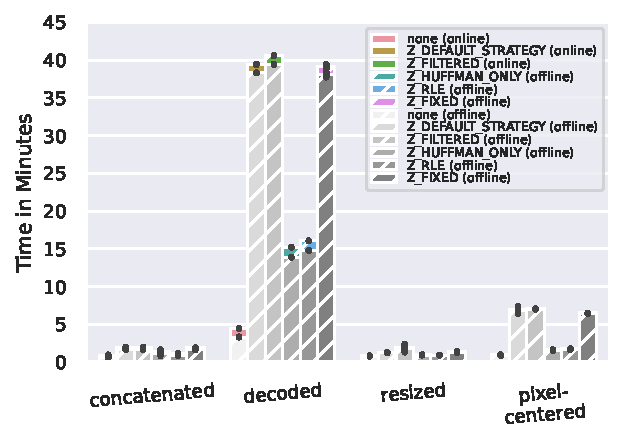
\includegraphics[width=\linewidth]{../images/cubeplusplus-jpg-strategy-pipeline/compression-processing-time-split.pdf}
    \caption{Cube++ - JPG}
    \Description{}
    \label{fig:zlib-cpp-jpg-compression-processing-time-split}
  \end{subfigure}
  
  % PNG
  \begin{subfigure}{0.49 \columnwidth}
    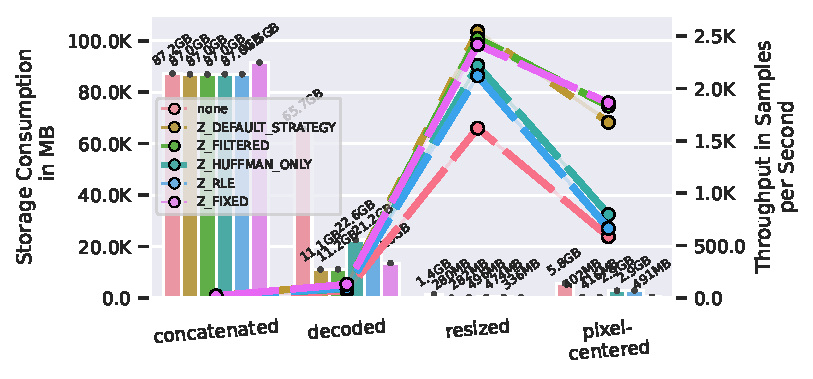
\includegraphics[width=\linewidth]{../images/cubeplusplus-png-strategy-pipeline/compressed-storage-vs-throughput.pdf}
    \caption{Cube++ - PNG}
    \Description{}
    \label{fig:zlib-cpp-png-compressed-storage-vs-throughput}
  \end{subfigure}
  \hfill %%
  \begin{subfigure}{0.49 \columnwidth}
    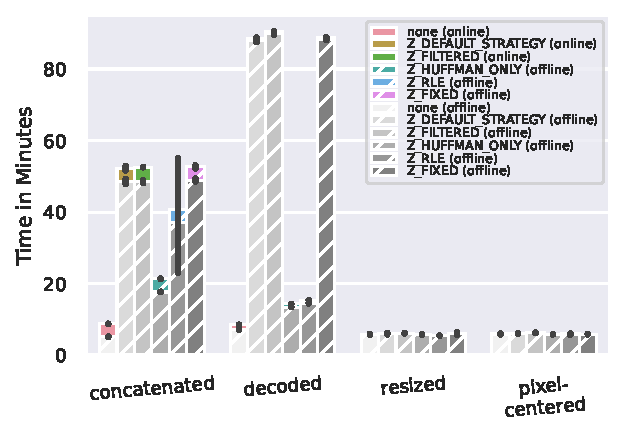
\includegraphics[width=\linewidth]{../images/cubeplusplus-png-strategy-pipeline/compression-processing-time-split.pdf}
    \caption{Cube++ - PNG}
    \Description{}
    \label{fig:zlib-cpp-png-compression-processing-time-split}
  \end{subfigure}
  
  % librispeech
  \begin{subfigure}{0.49 \columnwidth}
    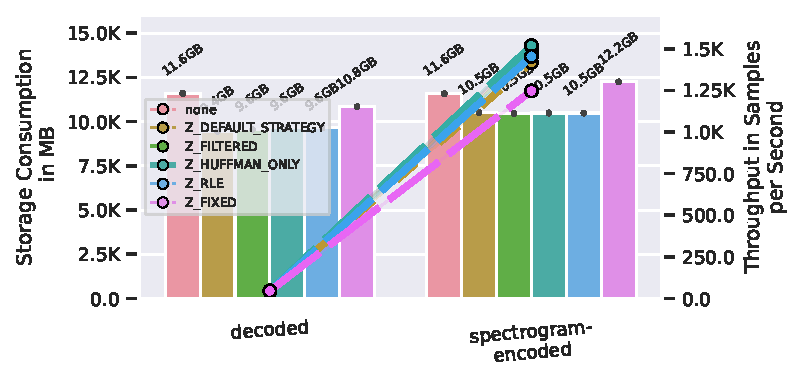
\includegraphics[width=\linewidth]{../images/librispeech-strategy-pipeline/compressed-storage-vs-throughput.pdf}
    \caption{Librispeech}
    \Description{}
    \label{fig:zlib-librispeech-compressed-storage-vs-throughput}
  \end{subfigure}
  \hfill %%
  \begin{subfigure}{0.49 \columnwidth}
    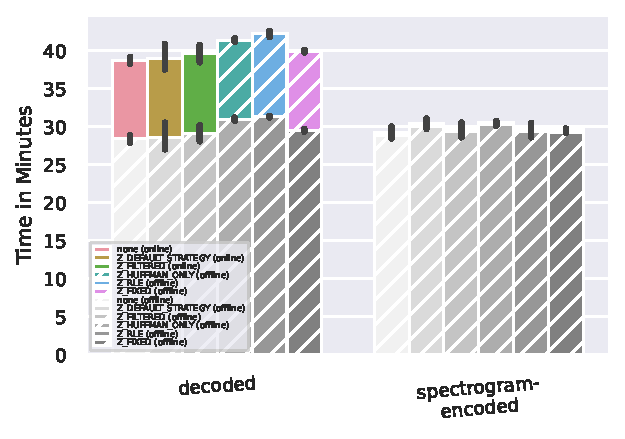
\includegraphics[width=\linewidth]{../images/librispeech-strategy-pipeline/compression-processing-time-split.pdf}
    \caption{Librispeech}
    \Description{}
    \label{fig:zlib-librispeech-compression-processing-time-split}
  \end{subfigure}
  
  % commonvoice
  \begin{subfigure}{0.49 \columnwidth}
    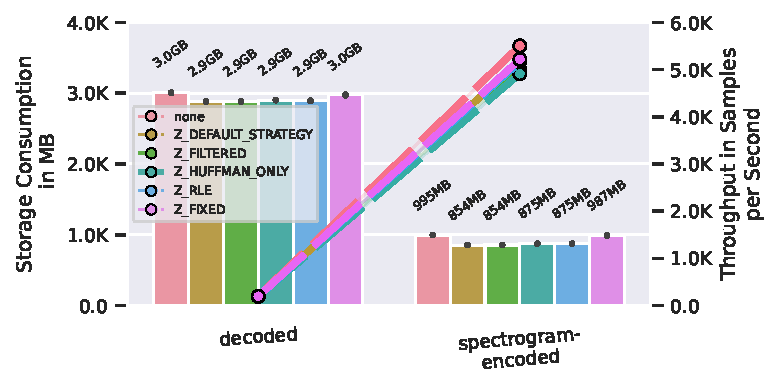
\includegraphics[width=\linewidth]{../images/commonvoice-strategy/compressed-storage-vs-throughput.pdf}
    \caption{Commonvoice}
    \Description{}
    \label{fig:zlib-strategy-commonvoice-compressed-storage-vs-throughput}
  \end{subfigure}
  \hfill %%
  \begin{subfigure}{0.49 \columnwidth}
    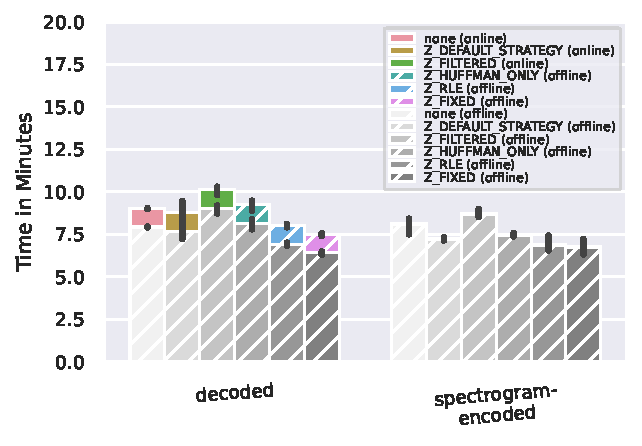
\includegraphics[width=\linewidth]{../images/commonvoice-strategy/compression-processing-time-split.pdf}
    \caption{Commonvoice}
    \Description{}
    \label{fig:zlib-strategy-commonvoice-compression-processing-time-split}
  \end{subfigure}
  
  \caption{(ZLIB) \textbf{Left column}: storage consumption compared to throughput. \textbf{Right column}: offline (gray bars) and online processing time (colored bars) with compression.}
  \label{fig:zlib-experiments}
\end{figure}

\subsection{Zstandard}
By default, Zstandard is not integrated into TensorFlow.
For this reason, we had to extend TensorFlow's codebase to include Zstandard, in particular, its advanced streaming compression API.
No support for multithreading has been added for now, due to the elevated complexity of integrating it into TensorFlow.
After constructing a successful implementation, we analyzed its performance against no compression, ZLIB using \texttt{Z\_DEFAULT\_STRATEGY} and GZIP.
We make the following observations based on \autoref{fig:zstd-experiments}:

\textbf{(1) ZSTD runs much faster in certain scenarios, but not always}.
Running tests on Cube++ showed that the use of Zstandard improved execution times significantly in both JPEG and PNG scenarios.
ZLIB and GZIP are quite slow, taking up to 9x as much as no compression at all (see \autoref{fig:zstd-cpp-png-compression-processing-time-split}).
Zstandard on the other hand takes only 1.5x as much as no compression.
However, this speedup is not consistent across other datasets.
In fact, Zstandard is slower than no compression, ZLIB, and GZIP in Librispeech and Commonvoice.
As noted by \cite{isenko2022bottleneck}, this may be due to a CPU bottleneck 

\textbf{(2) Compression ratio is similar to ZLIB and GZIP}.
In our tests, we observed that storage savings for ZSTD don't diverge from the average of other compression algorithms.
Actually, Zstandard does not aim to provide a better compression ratio than ZLIB or GZIP and instead focuses more on compression and decompression speed.

\textbf{(3) Compression ratio is not a reliable predictor of throughput}.
Again, we observe how the compression ratio does not seem to predict throughput in every scenario.
The compression ratio then should not be taken into consideration when selecting which compression algorithm to choose to obtain higher throughput.

\textbf{(5) Throughput is similar to GZIP and ZLIB}.
Looking at previous observations, we noticed how throughput for Zstandard has remained almost unchanged with respect to ZLIB and GZIP.
This is curious, as we expected that with much faster compression and decompression also came higher throughput.
In fact, throughput for Zstandard runs can be a bit lower than ZLIB and GZIP.


\begin{figure}[b]
  %JPG
  \begin{subfigure}{0.49 \columnwidth}
    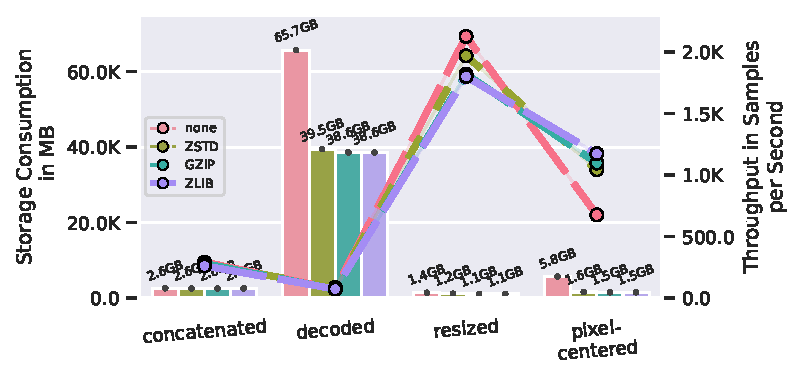
\includegraphics[width=\linewidth]{../images/cubeplusplus-jpg-pipeline/compressed-storage-vs-throughput.pdf}
    \caption{Cube++ - JPG}
    \Description{}
    \label{fig:zstd-cpp-jpg-compressed-storage-vs-throughput}
  \end{subfigure}
  \hfill %%
  \begin{subfigure}{0.49 \columnwidth}
    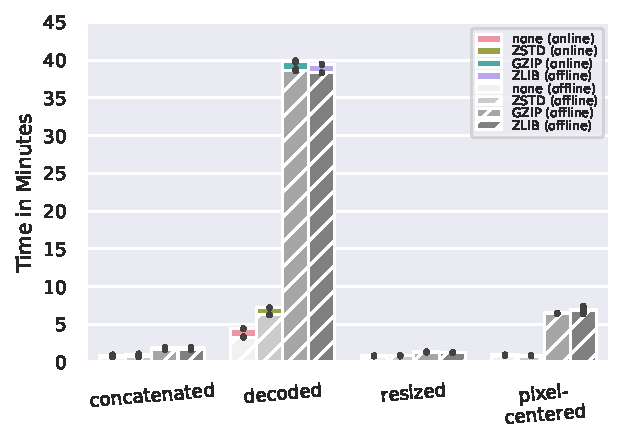
\includegraphics[width=\linewidth]{../images/cubeplusplus-jpg-pipeline/compression-processing-time-split.pdf}
    \caption{Cube++ - JPG}
    \Description{}
    \label{fig:zstd-cpp-jpg-compression-processing-time-split}
  \end{subfigure}
  
  % PNG
  \begin{subfigure}{0.49 \columnwidth}
    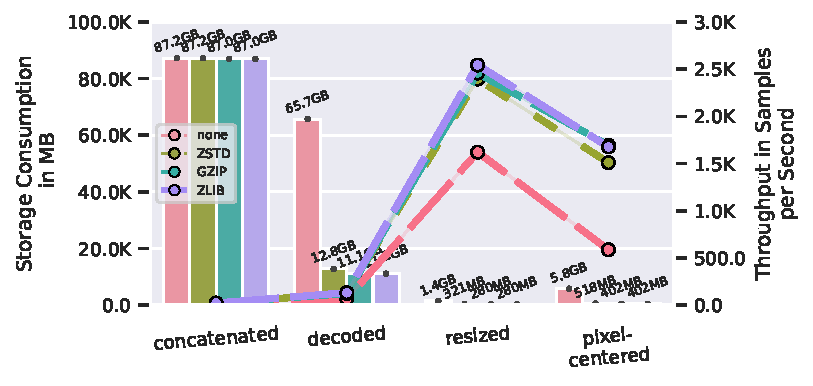
\includegraphics[width=\linewidth]{../images/cubeplusplus-png-pipeline/compressed-storage-vs-throughput.pdf}
    \caption{Cube++ - PNG}
    \Description{}
    \label{fig:zstd-cpp-png-compressed-storage-vs-throughput}
  \end{subfigure}
  \hfill %%
  \begin{subfigure}{0.49 \columnwidth}
    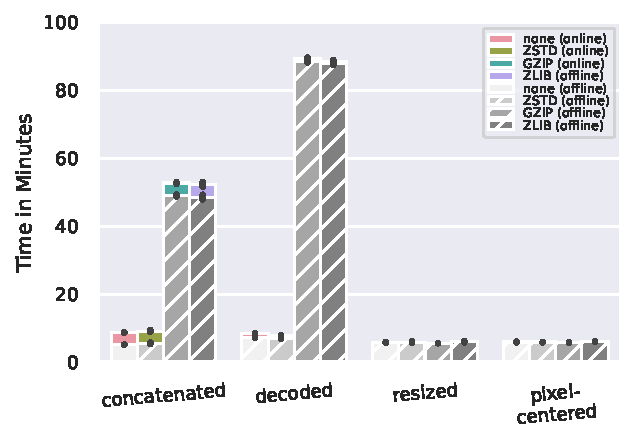
\includegraphics[width=\linewidth]{../images/cubeplusplus-png-pipeline/compression-processing-time-split.pdf}
    \caption{Cube++ - PNG}
    \Description{}
    \label{fig:zstd-cpp-png-compression-processing-time-split}
  \end{subfigure}
  
  % librispeech
  \begin{subfigure}{0.49 \columnwidth}
    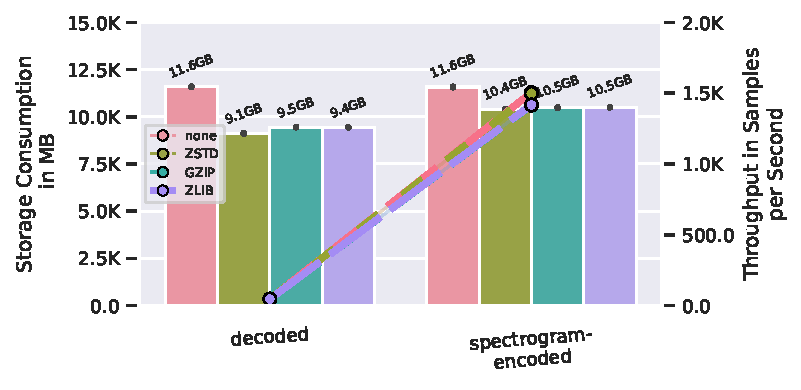
\includegraphics[width=\linewidth]{../images/librispeech-pipeline/compressed-storage-vs-throughput.pdf}
    \caption{Librispeech}
    \Description{}
    \label{fig:zstd-librispeech-compressed-storage-vs-throughput}
  \end{subfigure}
  \hfill %%
  \begin{subfigure}{0.49 \columnwidth}
    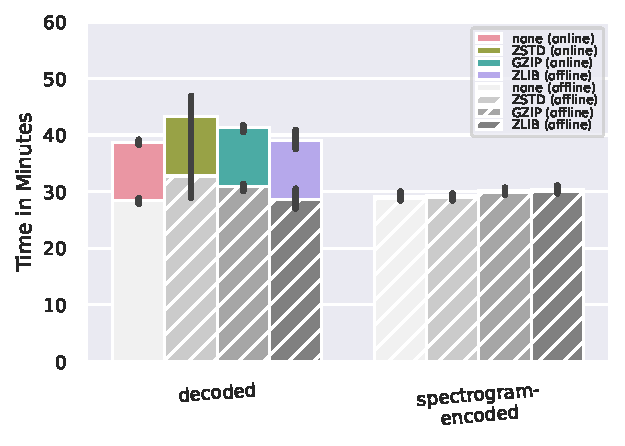
\includegraphics[width=\linewidth]{../images/librispeech-pipeline/compression-processing-time-split.pdf}
    \caption{Librispeech}
    \Description{}
    \label{fig:zstd-librispeech-compression-processing-time-split}
  \end{subfigure}
  
  % commonvoice
  \begin{subfigure}{0.49 \columnwidth}
    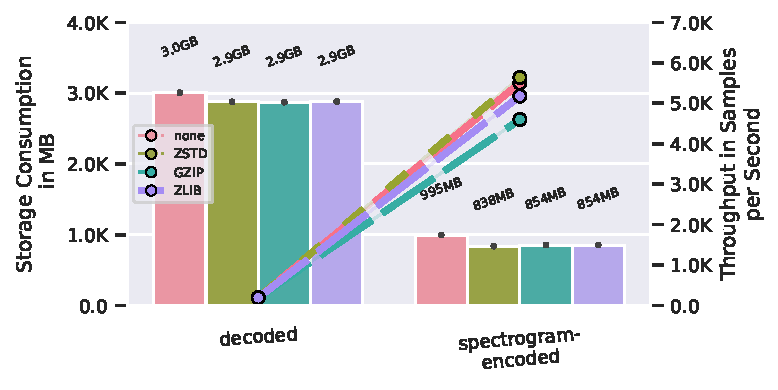
\includegraphics[width=\linewidth]{../images/commonvoice-pipeline/compressed-storage-vs-throughput.pdf}
    \caption{Commonvoice}
    \Description{}
    \label{fig:zstd-commonvoice-compressed-storage-vs-throughput}
  \end{subfigure}
  \hfill %%
  \begin{subfigure}{0.49 \columnwidth}
    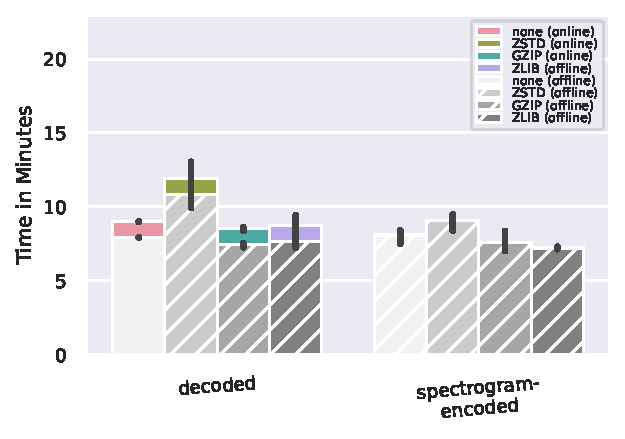
\includegraphics[width=\linewidth]{../images/commonvoice-pipeline/compression-processing-time-split.pdf}
    \caption{Commonvoice}
    \Description{}
    \label{fig:zstd-commonvoice-compression-processing-time-split}
  \end{subfigure}
  
  \caption{(ZSTD) \textbf{Left column}: storage consumption compared to throughput. \textbf{Right column}: offline (gray bars) and online processing time (colored bars) with compression.}
  \label{fig:zstd-experiments}
\end{figure}

\begin{figure}
  \begin{subfigure}{0.49 \columnwidth}
    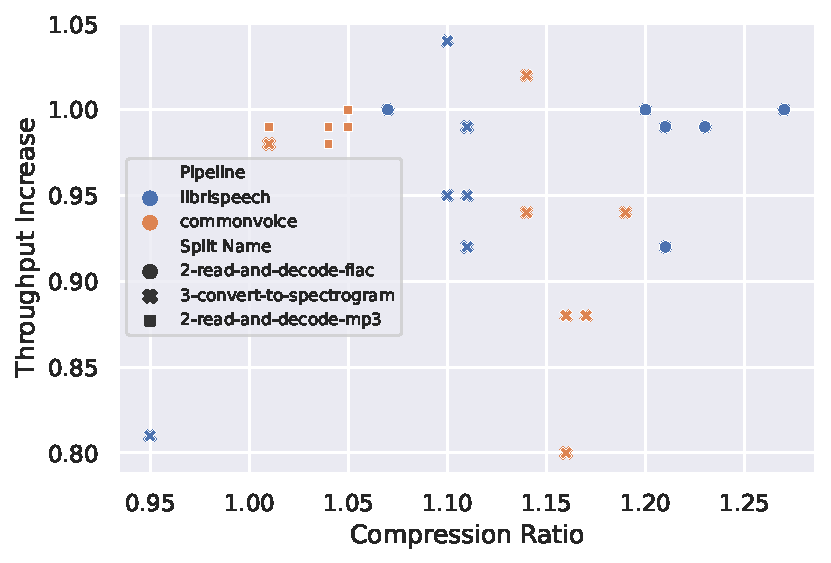
\includegraphics[width=\linewidth]{../images/compression-ratio-vs-throughput/librispeech-commonvoice-compression-ratio-vs-throughput.pdf}
    \caption{Librispeech and Commonvoice}
    \Description{}
    \label{fig:librispeech-commonvoice-compression-ratio-vs-throughput}
  \end{subfigure}
  \hfill %%
  \begin{subfigure}{0.49 \columnwidth}
    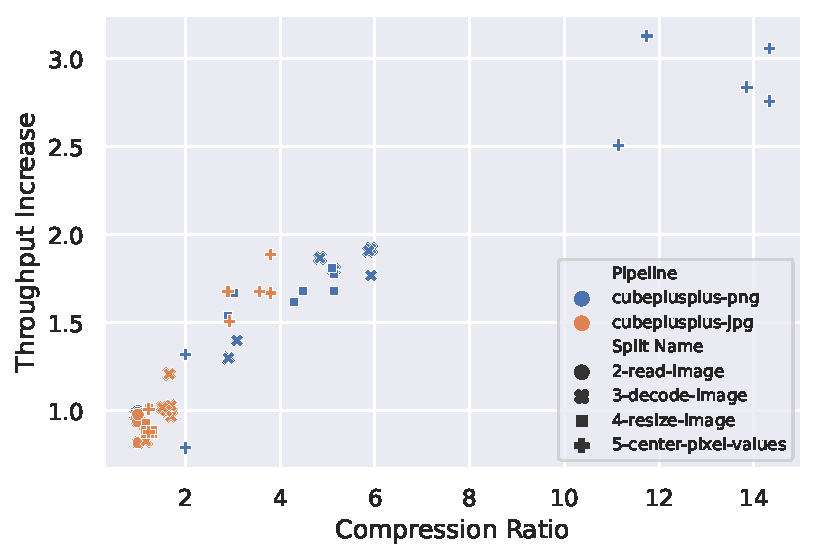
\includegraphics[width=\linewidth]{../images/compression-ratio-vs-throughput/cubeplusplus-compression-ratio-vs-throughput.pdf}
    \caption{Cube++}
    \Description{}
    \label{fig:cubeplusplus-compression-ratio-vs-throughput}
  \end{subfigure}
  \caption{Relation between compression ratio and throughput increase for Librispeech, Commonvoice and Cube++.
    Colors represent the dataset, shapes represent the name of the steps.
    We group the data according to the similarity between pipelines.
    Both Cube++ pipelines seem to have a linear relationship between compression ratio and throughput increase.
    Librespeech and Commonvoice do not show any particular pattern.}
  \Description{}
  \label{fig:compression-ratio-vs-throughput}
\end{figure}

\section{Conclusions}
In this paper, we have extended the observations made by \citet{isenko2022bottleneck} with respect to the effects of compression algorithms in preprocessing pipelines.
We ran the PRESTO profiler on a virtual machine with similar characteristics and on the same datasets, except Openwebtext and ImageNet, using Zstandard and different compression strategies for ZLIB.
For ZLIB, we found that some compression strategies provide slightly better throughput compared to the \texttt{Z\_DEFAULT\_STRATEGY} and no compression, in particular when dealing with PNG images.
Furthermore, some strategies execute faster than both the default strategy and no compression at all under certain scenarios, with no reduction in throughput.

Zstandard performed significantly better in terms of execution time on Cube++, both JPG and PNG pipelines.
However, we didn't find any particular improvement in throughput compared to other compression strategies such as ZLIB and GZIP, sometimes even showing a reduction in throughput.
We suggest replacing the use of ZLIB or GZIP with Zstandard as a compression algorithm where the throughput is comparable, and Zstandard presents computational time overhead.

We observed that compression ratio seems to be positively correlated when dealing with Cube++, for both PNG and JPEG images, as shown by \autoref{fig:compression-ratio-vs-throughput}, regardless of the compression algorithm of choice.
On the other hand, throughput for Librispeech and Commonvoice does not seem to be affected by compression ratio in the same way as Cube++ pipelines.
This effect is already documented by \cite{isenko2022bottleneck}, pointing to CPU bottlenecks.

No compression algorithm is the same.
Our work shows that introducing compression in data preprocessing pipelines must be done with care.
As each pipeline and step have different properties, one must then select compression algorithms accordingly.

\section{Future Work}
In this work, we have decided to use the opinionated \texttt{TFRecord} data format for TensorFlow.
However, data formats with multi-framework support already exist:

WebDataset \cite{aizman2020highperformance} for example uses the old data archive format TAR.
Although TAR supports different compression algorithms \footnote{gzip, bzip2, xz, lzip, lzma, lzop, zstd}, their work does not make use of it.
Instead, they support compression of single image files using the Pillow \footnote{https://pypi.org/project/Pillow/} package.
In the future, we may want to replicate our findings using WebDataset by adding compression to TAR files.
FFCV by \citet{leclerc2022ffcv} is a data loading system that has been recently published, and it has reported huge speedups in the preprocessing pipeline.
The framework does not mention or support the use of compression.
This lack of support opens up further research possibilities in this area, possibly further improving preprocessing pipeline speeds.

\texttt{DEFLATE}, the algorithm upon which both ZLIB and GZIP are based, was developed in 1996, and has remained virtually unchanged since then.
Zstandard was developed in 2015 by Facebook with more modern hardware in mind and is able to exploit multithreading using its streaming API.
Our implementation does not make use of the multithreading, and in future work, it may be possible to further modify our implementation to introduce it.

In this paper, we have observed how the presence of certain components in a compression algorithm such as string matching can affect both consumption speed and throughput.
It might be beneficial to develop a compression algorithm that combines several of these components, turning them on or off depending on the data properties.
For example, \citet{burtscher2010gfpc} introduces gFPC, a self-tuning compression algorithm for floating-point data.
When executing operations inside a GPU, swapping tensors can be an expensive task.
\citet{chen2021cswap} address this issue with CSWAP, dynamically choosing between four compression algorithms: zero-value compression (ZVC) \cite{rhu2018compressing}, Run-Length Encoding (RLE) \cite{robinson1967results}, Compressed Sparse Row (CSR) \cite{alabaichi2017anovel} and LZ4.

Using different lossless data formats can help reduce storage consumption footprint and speed up the preprocessing pipeline.
The Quite OK (QOI) \cite{qoi2021dominic} data format has recently received a lot of attention in this regard, claiming 20x-50x faster encoding and 3x-4x faster decoding with respect to PNG, while offering a similar compression ratio.
It can also be paired with other compression algorithms to achieve possibly achieve a higher compression ratio for limited storage scenarios.
Other attempts to have dedicated data formats exist, such as DeepN-JPEG \citet{liu2018deepn-jpeg}, a format based on JPEG but dedicated to deep learning environments.

Until now, we have only taken a look at lossless compression algorithms.
However, there might be even more advantages in using lossy compression algorithms instead, without necessarily sacrificing accuracy or training time.
ZFP \cite{lindstorm2014fixedrate} is a lossy compression algorithm for n-dimensional floating-point data, with options for error-bounding the compression.
In general, lossy compression algorithms may be used to reduce storage consumption and have been shown to maintain similar accuracy scores \cite{liu2018deepn-jpeg, dodge2016understanding}.

\bibliographystyle{ACM-Reference-Format}
\bibliography{report}

\end{document}
